\section{Evaluation}
\label{sec:6}
We demonstrate that SilverTorch offers performance improvement with better cost-efficiency. We also show that SilverTorch enables more complex architectures that improves retrieval recalls. Our experiments use the real-world dataset sampled from production. The dataset consists of a candidate pool of 80 million items(referred to as 80M-dataset) and a candidate pool of 10 million items(referred to as 10M-dataset). 
We set the embedding dimensions to 128 for experiments. We reuse the model architecture to evaluate performance and use A100 40G GPUs. The replayed requests are generated from real traffic containing 5000 recommendation requests. For the end-to-end experiments, we measure Query per Second(QPS) from client side given 200 ms  P99 latency budget. We observe that given more small latency budget, the throughput number of the CPU baselines is too small to report. The client concurrently sends requests to predictor and indexing servers. For each test, we gradually increase sending QPS to avoid server-side congestion and report the maximum throughput it could reach. Each experiment is running 5 times and we report the average. To evaluate the OverArch and in-model Value Model, we measure recalls at different scales, together with QPS.

\underline{Baseline-Retrieval} is a service-based retrieval system. The client first sends a request to predictor that serves User Tower on 1 GPU and gets the user embedding. The client sends user embedding with filtering queries to indexing servers. The indexing servers contain ANN search index built based on the Faiss-CPU(IVF) and inverted-index(CPU) for feature filtering. Each inverted-index server builds its index on a partition of items and the filtering queries are running in a scatter-gather manner. \underline{Baseline-Retrieval-GPU} is a service-based retrieval baseline on GPUs. User Tower is served on 1 GPU. The ANN search index is built based on Faiss-GPU(IVF) and the filtering index is using GPU-based forward index discussed in \ref{sec:4.1}. The ANN index and the forward index are served in multiple GPUs. Each GPU builds its index on a partition of items, the ANN search and filtering are running in a scatter-gather manner. 1 means no sharding. \underline{SilverTorch-Retrieval} is the SilverTorch retrieval without OverArch and Value Model layers. Client sends a single request to GPU predictor. The server computes the user embedding followed by SilverTorch's co-designed ANN search and bloom index, returning topk item ids. For the end-to-end experiments, we shard it to 2 GPUs for 80M-dataset and use a single GPU for 10M-dataset. \underline{SilverTorch-Retrieval-OverArch} is SilverTorch retrieval with OverArch scoring layer and the in-model Value Model. This is the multi-task setup. We compare SilverTorch's ANN with Faiss-CPU(IVF), Faiss-GPU(IVF) and HNSW. We compare Bloom Index with the GPU-based forward index and the CPU-based inverted index.

\begin{figure*}[h]
    \centering
    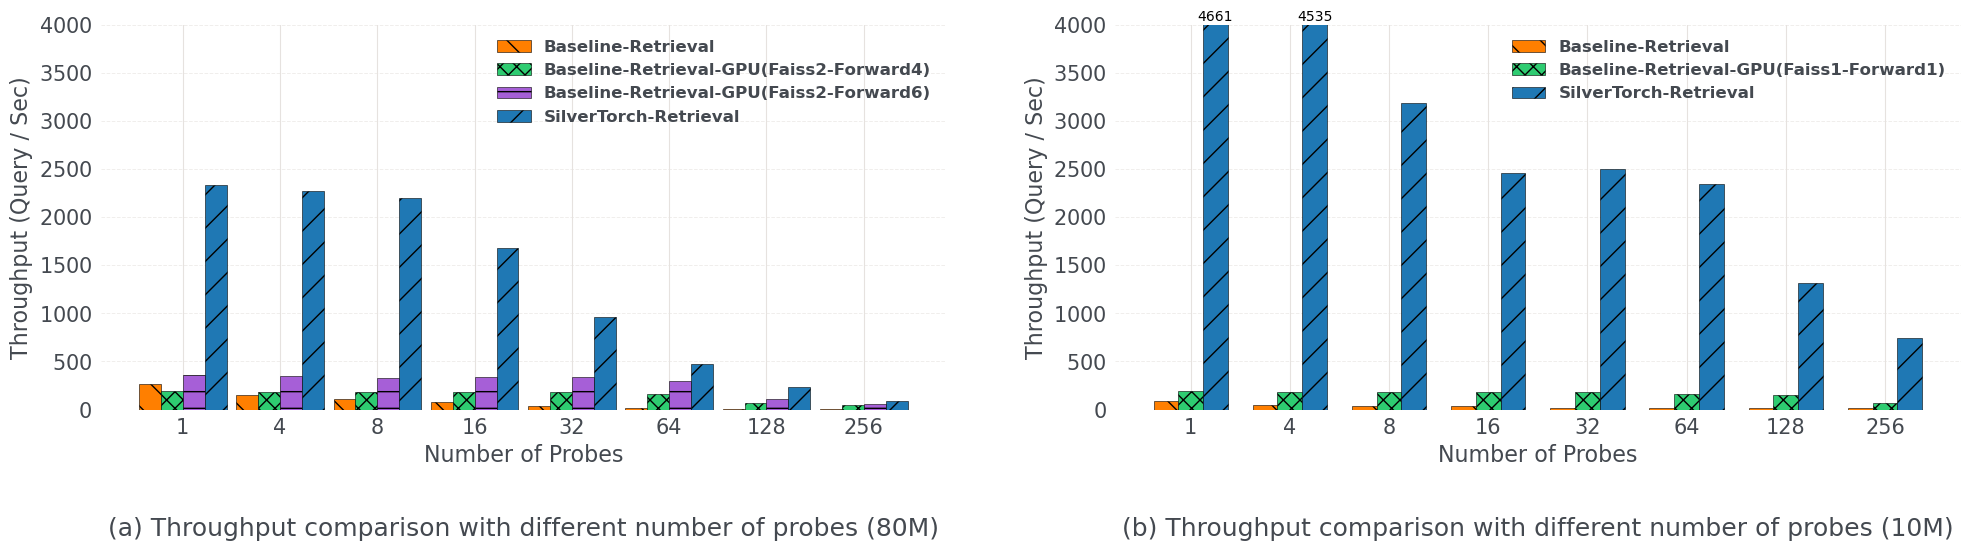
\includegraphics[width=1.0\textwidth]
    {figures/exp/experiment_e2e_final2.png}
    \caption{End-to-end performance Results for Retrieval.}
    \label{fig:retrieval-e2e}
\end{figure*}

\subsection{End-to-end Evaluation}
\subsubsection{Throughput}
\label{sec:611}
We build the state-of-the-art CPU-based baseline adopting the same model architecture. It is a multi-task model with 12 embedding heads per user, performing 12-way top-k ANN search. Filtering queries combine AND/OR/NOT operators across 6 features with 7 conditions on average, using Faiss-CPU for ANN and our internal inverted index implementation. For the 80M dataset, indexes are sharded across 2 CPU servers (Faiss) and 4 servers (inverted index)—the minimal configuration for meaningful QPS. Requests fan out to shards and merge at an aggregator. The 10M dataset runs un-sharded.
Figure \ref{fig:retrieval-e2e} shows end-to-end performance varying ANN probes with top-k fixed at 1024. Faiss-CPU uses 64 OpenMP threads. GPU baselines are labeled FaissX-ForwardY, indicating X Faiss shards and Y forward index shards.
For the 80M dataset (40GB memory requiring 2 Faiss-GPU shards) at 24 probes(production setting), SilverTorch achieves 1210 QPS—$23.7\times$ over CPU baseline and $3.5\times$–$6.7\times$ over GPU baselines. Although GPU baseline performance improves with more shards, cost increases linearly.
For the 10M dataset without sharding, SilverTorch achieves 3802 QPS—$165.3\times$ over CPU and $20.8\times$ over GPU baselines. Notably, SilverTorch QPS scales $3.1\times$ when reducing pool size from 80M to 10M, while baseline QPS remains similar since per-server item count is unchanged.

\begin{table}[t]
  \centering
  \caption{Cost-efficiency Breakdowns}
  \label{tab:TCO-analysis}
  \resizebox{0.5\textwidth}{!}{
  \begin{tabular}{ccccc}
    \toprule
    Baselines & QPS & TCO/Hour & TCO/1000 Requests & Cost Efficiency\\
    \midrule
    Baseline-CPU & 51 & \$28.92 & \$0.158 & 1 \\
    Baseline-GPU(Faiss2-Forward4) & 186 & \$30.29 & \$0.0452 & $3.48\times$ \\
    Baseline-GPU(Faiss2-Forward6) &  340 & \$33.27 & \$0.0272 & $5.8\times$ \\
    SilverTorch & 1210 & \$33.27 & \$0.0077 & $20.9\times$ \\
    SilverTorch-OverArch & 771 & \$33.27 & \$0.012 & $13.35\times$ \\
    \bottomrule
    \end{tabular}
}
\end{table}

\subsubsection{Cost Efficiency Analysis}
To illustrate the cost efficiency of SilverTorch, we estimate Total Cost of Ownership (TCO) reduction using QPS results from the 80M-dataset experiments. Our CPU server has 256GB memory and 40 cores, while GPU servers have 48 CPU cores, 384GB memory, and varying numbers of A100 40GB cards. We map these to similar AWS instance types to estimate TCO.
For the CPU server, we use r6i.8xlarge (32 vCPUs, 256GB memory) at 2.24/hour~\cite{r6i8xlarge} as a lower-bound estimate. For GPU servers, AWS offers A100 40GB exclusively in p4d.24xlarge instances with 8 GPU cards, 96 vCPUs, and 1.15TB memory at 32.77/hour. To estimate the cost of a single A100 40GB card, we subtract the CPU-equivalent cost (x2idn.24xlarge at 13.01/hour~\cite{x2idn24xlarge}) and divide by 8, yielding 2.47/hour per GPU. Thus, the baseline's user tower with one GPU costs approximately 15.47/hour.
Using the QPS results, we evaluate cost efficiency as follows. Baseline-Retrieval uses one GPU for user tower, 2 CPU servers for ANN search, and 4 CPU servers for filtering, totaling 28.92/hour with 51 QPS. The GPU baselines Baseline-Retrieval-GPU-Faiss2-Forward4 and Baseline-Retrieval-GPU-Faiss2-Forward6 cost 30.29 and 32.77/hour, achieving 184 and 340 QPS respectively. SilverTorch-Retrieval uses one GPU server with 2 A100 40GB cards at 32.77/hour~\cite{p4d24xlarge}, achieving 1210 QPS.
Table \ref{tab:TCO-analysis} shows the TCO breakdown for serving traffic at 1000 QPS. SilverTorch achieves $20.9\times$ cost-efficiency improvement over CPU baseline and $3.56\times$ over the best GPU baseline. Furthermore, when including computational overhead of OverArch and Value Model, SilverTorch's QPS decreases to 771, which still delivers $13.35\times$ improvement over CPU solution and $2.27\times$ over GPU solution.

%To illustrate cost efficiency of SilverTorch's GPU solution, we estimate  reduction of Total Cost of Ownership(TCO) using the QPS results from 80M-dataset experiments. For the CPU server we use the machine with 256GB memory and 40 Cores. For the GPU server, we use the machine with 48 CPU Cores and 384GB Memory with different numbers of A100 40GB cards. We find the similar instance types in AWS to estimate TCO. AWS does not have EC2 instance with identical configuration, therefore we find close instance types to estimate the lower bound. Specifically, we estimate TCO of our CPU server using r6i.8xlarge(32 vCPUs, 256GB Memory) in the region of US West, the rate is around \$2.24/hour~\cite{r6i8xlarge} for on-demand plan. For GPU servers, AWS only offers A100 40GB exclusively in p4d.24xlarge instances, each consisting of 8 GPU cards, 96 vCPUs and 1.15 TB Memory at the rate of \$32.7726/hour~\cite{p4d24xlarge} for on-demand plan. We use this number to estimate the TCO per hour for SilverTorch and GPU baseline. Meanwhile, to project to the cost with a single A100 40G GPU card for baseline's user tower, we find similar CPU configuration of the GPU server, which is x2idn.24xlarge~\cite{x2idn24xlarge} and its rate is \$13.005/hour. Therefore, a single A100 40G GPU's TCO per hour can be estimated as $\frac{(\$32.7726-\$13.005)}{8}=\$2.47$. We estimate the TCO per hour for baseline's user tower to be $\$13.005 + \$2.47 = \$15.47$.
%We use the previous QPS results to evaluate the cost efficiency.
%The Baseline-Retrieval uses one GPU to serve user tower and uses 2 CPU servers to serve ANN search and 4 CPU servers to serve filtering. Therefore, the TCO of Baseline-Retrieval per hour is $\$15.47+\$2.24*(2+4)=\$28.92$. \blue{The TCO of Baseline-Retrieval-GU-Faiss2-Forward4 and Baseline-Retrieval-GU-Faiss2-Forward6 per hour are $\$15.47+\$2.47*(2+4)=\$30.29$ and $32.77$ respectively. The SilverTorch-Retrieval is using one GPU server of two A100 40G cards, contributing two the total TCO per hour is up to $\$32.77$. To serve the same amount of queries, considering the QPS of Baseline-Retrieval, two GPU baselines are 51, 184 and 340 respectively}, while the QPS of SilverTorch-Retrieval is 1210. Table \ref{tab:TCO-analysis} shows breakdown TCO for serving a traffic with QPS of 1000. \blue{SilverTorch achieves $\frac{1210}{340}*\frac{28.92}{33.27} = 20.9\times$ cost-efficiency speedups comparing to CPU-based baseline and $3.56\times$ speedups comparing to the best GPU-based baseline}.
%Furthermore, considering the recall wins brings from SilverTorch's OverArch and value mode, the QPS decreases to 771, which still has $13.35\times$ improvement than CPU-based solution and $2.27\times$ improvement than GPU-based solution.

\subsection{Breakdown Analysis}
In this section, we evaluate the performance of each component in SilverTorch. We focus on a single GPU experiments.

\subsubsection{Evaluation on ANN Search}
\begin{figure}
    \centering
    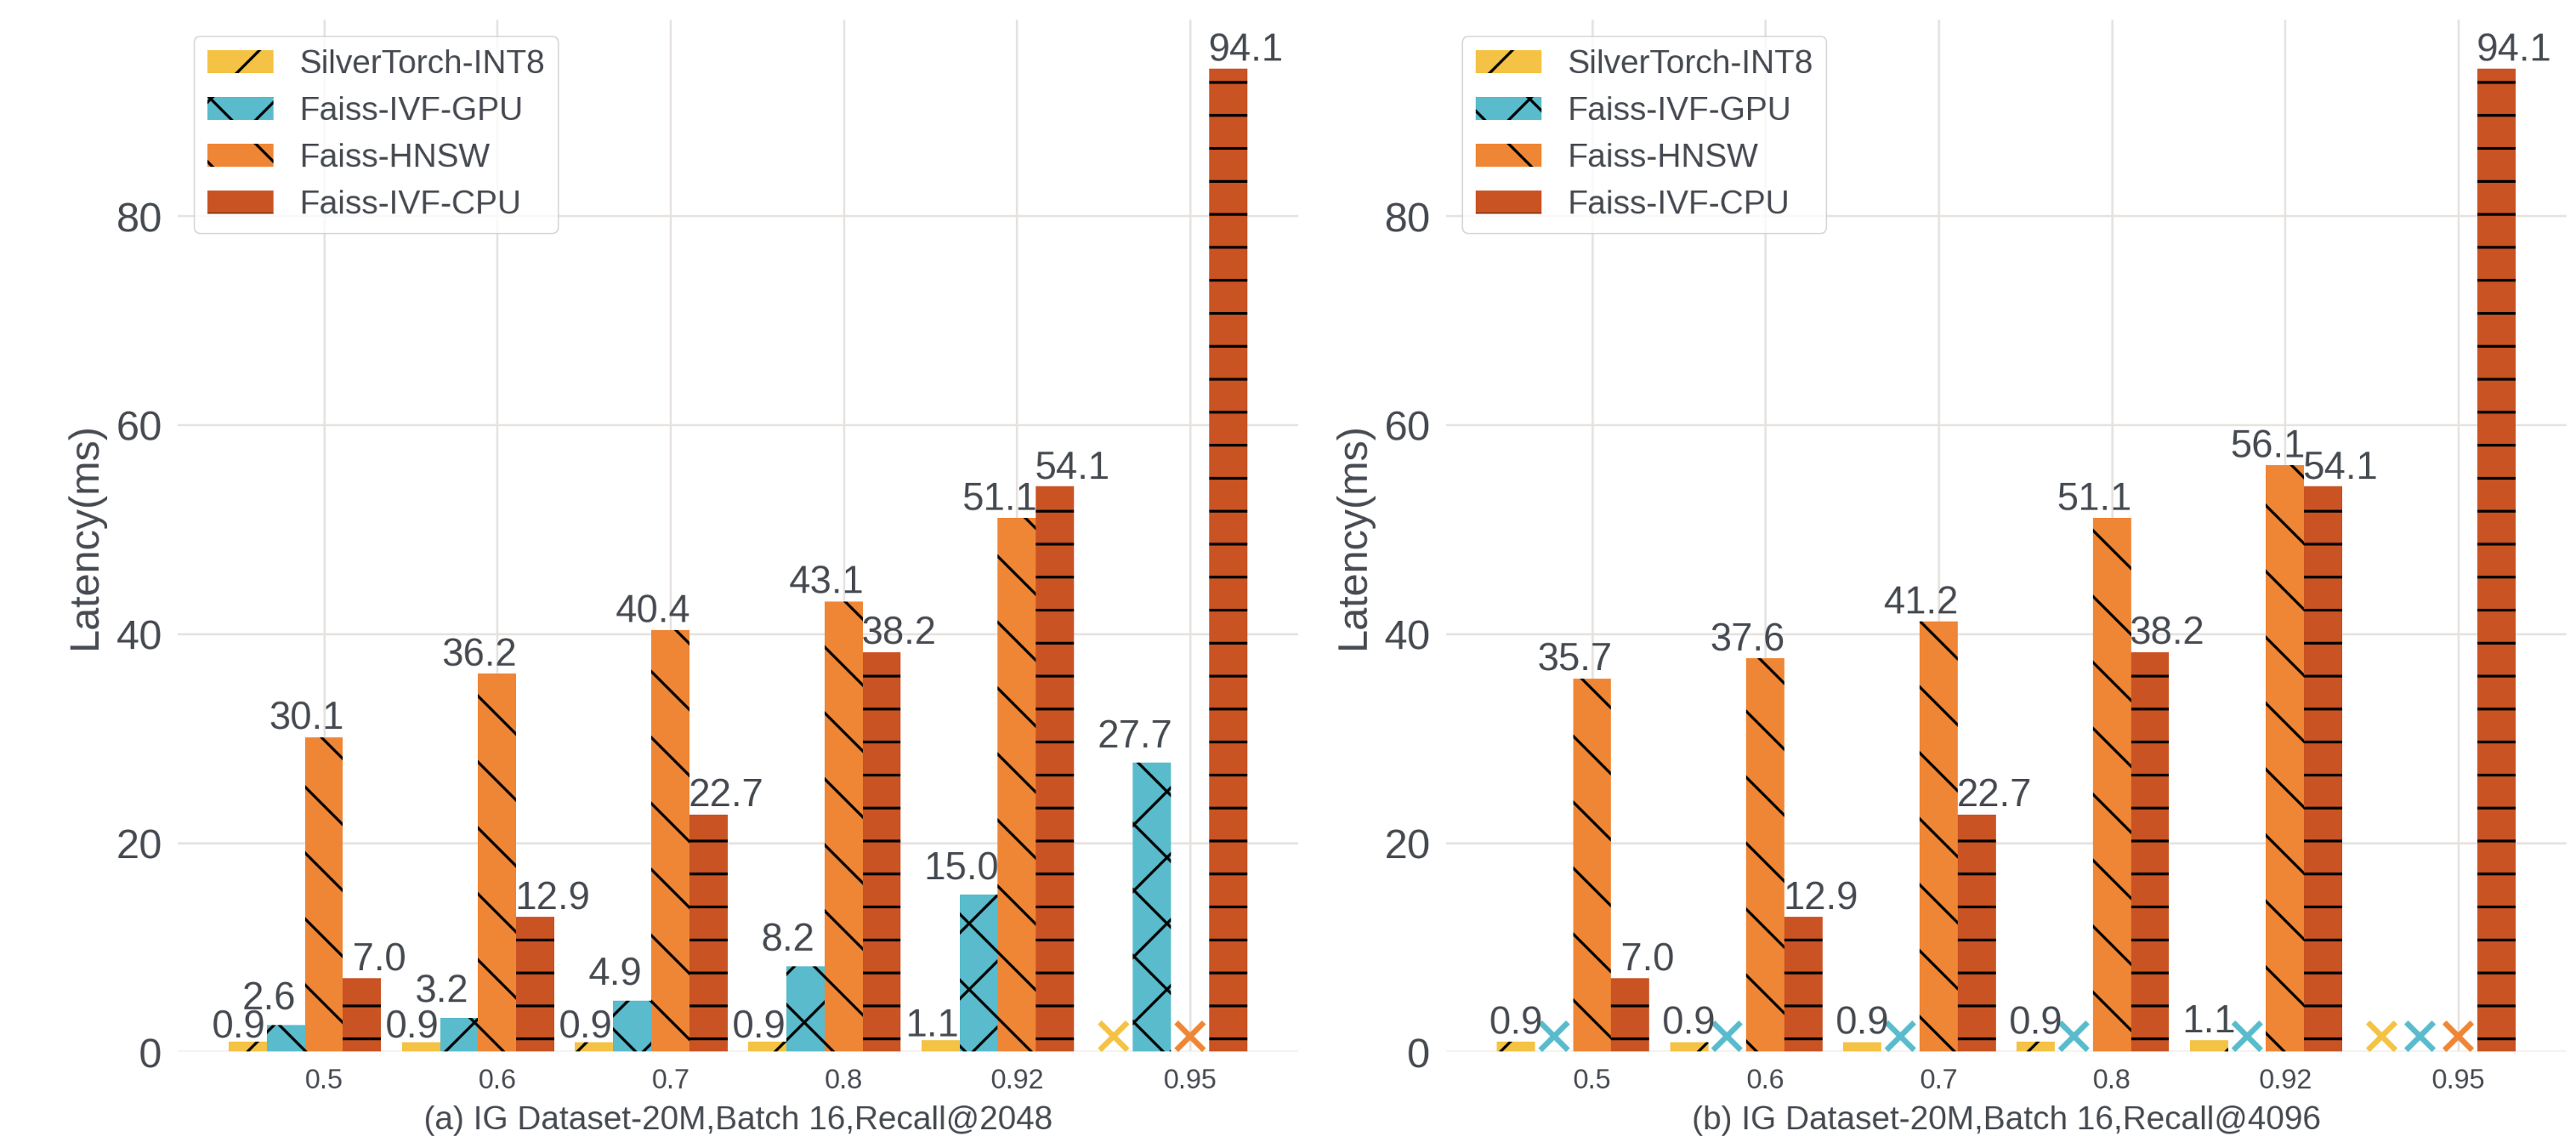
\includegraphics[width=0.5\textwidth]
    {figures/exp/ann_latency_recall2.png}
    \caption{Latency/Recall results of different ANN methods.}
    \label{fig:ann_latency_recall}
\end{figure}

We compare SilverTorch's ANN search against both CPU and GPU baselines. For Faiss, we evaluate the most efficient IVFFlat index with float32 on both CPU and GPU, as well as HNSW. CAGRA(GPU) limits top-k to 1024, making it unsuitable for recommendation scenarios for comparison.
Since HNSW is graph-based without a probes parameter, we compare average latency at equivalent recall levels. The dataset contains 20 million item embeddings with 128 dimensions, with query embeddings generated from the User Tower. We focus on single-server and single-GPU performance, running 50 warm-up batches followed by 100 test batches. While in practice we use top-k around 10,000, we test with 2048 and 4096 since Faiss-GPU only supports up to 2048.
Figure \ref{fig:ann_latency_recall} shows average latency across different recalls at batch size 16. SilverTorch-INT8 achieves the lowest latency in all cases. At top-k=2048, SilverTorch achieves $2.2\times$–$14.7\times$ lower latency than Faiss-GPU across recalls from 0.35 to 0.92. Due to INT8 quantization, SilverTorch cannot reach 0.95 recall. However, achieving this recall requires Faiss-CPU to use 1024 probes and Faiss-GPU to use 512 probes, which significantly degrades its performance. The latency savings from SilverTorch's ANN search can fund additional OverArch model computation.
At top-k=4096, Faiss-GPU cannot support it. SilverTorch-INT8 achieves $31.3\times$–$51\times$ lower latency than HNSW and $4.6\times$–$49.2\times$ lower latency than Faiss-CPU. Additionally, tuning cluster-based ANN is simpler(only probe parameter) comparing to HNSW's three interdependent parameters.

\begin{table*}[ht]
    \centering
    \small
    \begin{tabular}{llccccccc}
    \toprule
    \textbf{Task} & \textbf{Method} & \textbf{Recall@20} & \textbf{Recall@100} & \textbf{Recall@200} & \textbf{Recall@500} & \textbf{Recall@1000} & \textbf{QPS} \\
    \midrule
    \multirow{3}{*}{E-Task} 
        & Baseline & 0.08239 & 0.19179 & 0.29131 & 0.4295 & 0.44127 & 51 \\ 
        & SilverTorch & 0.07163 & 0.20306 & 0.28923 & 0.4237 & 0.44651 & 1210 \\ 
        & SilverTorch-OverArch & \textbf{0.09181 (+28.2\%)} & \textbf{0.24189 (+19.1\%)} & \textbf{0.33148 (+14.6\%)} & \textbf{0.44758 (+5.6\%)} & \textbf{0.45727 (+2.4\%)} & 771 \\ 
    \midrule
    \multirow{3}{*}{C-Task} 
        & Baseline & 0.09642 & 0.25217 & 0.3551 & 0.4971 & 0.5162 & 51 \\ 
        & SilverTorch & 0.09652 & 0.25291 & 0.352 & 0.4969 & 0.51973 & 1210 \\ 
        & SilverTorch-OverArch & \textbf{0.0971 (+0.6\%)} & \textbf{0.25733 (+1.7\%)} & \textbf{0.36011 (+2.3\%)} & \textbf{0.50747 (+2.2\%)} & \textbf{0.52559 (+1.12\%)} & 771 \\ 
    \bottomrule
    \end{tabular}
    \caption{Recall evaluations on a E-Task and a C-Task}
    \label{tab:recall-overarch}
\end{table*}

\subsubsection{Evaluation on Bloom Index}
We compare Bloom index performance against a production CPU inverted-index baseline and the forward index baseline on GPU. We evaluate on a single server with an index built on 40 million items, using 5,000 real filtering queries. Each item contains 6 features with 10 feature values on average. The Bloom index uses 5 hash functions.
Figure \ref{fig:bloom-all}(a) shows average latency per batch at different batch sizes. Bloom index supports batching more effectively, achieving $291\times$–$523\times$ speedup over inverted index and $12.6\times$–$42.7\times$ over forward index. Bloom index latency remains constant regardless of bit size (512 to 1024 bits), since queries involve a fixed number of hash functions and bitwise memory accesses that are efficiently parallelized via GPU warp-level execution. In contrast, inverted index latency varies significantly depending on posting list lengths.
Figure \ref{fig:bloom-all}(b) shows false positive rates at different bit sizes. Using 512 bits per item (1.2 GB total) yields 6.98 false positive rate, dropping to 0.067 at 1024 bits. The 512, 768, 1024, and 2048-bit configurations require 1.2, 1.8, 2.4, and 4.7 GB respectively. Inverted index requires 19.8 GB—$8.25\times$ larger than the 1024-bit Bloom index.
A heuristic for estimating optimal bit count is: maxfeaturevalues $\times$ hashfunctions $\times$ collisionbuffer. In our query set, with maximum 120 feature values per item, 5 hash functions, and buffer of 3, this yields 1800 bits per item.

\begin{figure}[h]
    \centering
    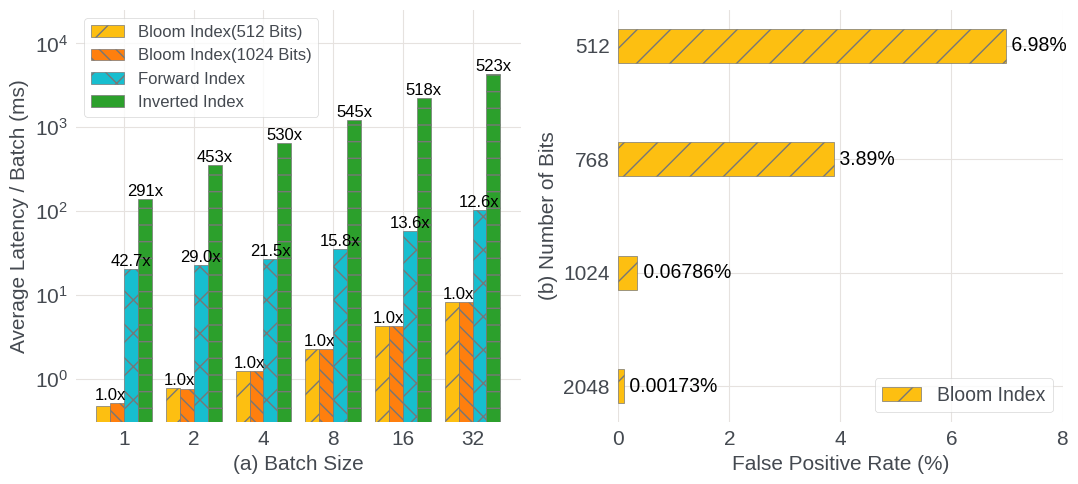
\includegraphics[width=0.5\textwidth]
    {figures/exp/bloom-all.png}
    \caption{Performance of Bloom Index.}
    \label{fig:bloom-all}
\end{figure}


\begin{figure}
    \centering
    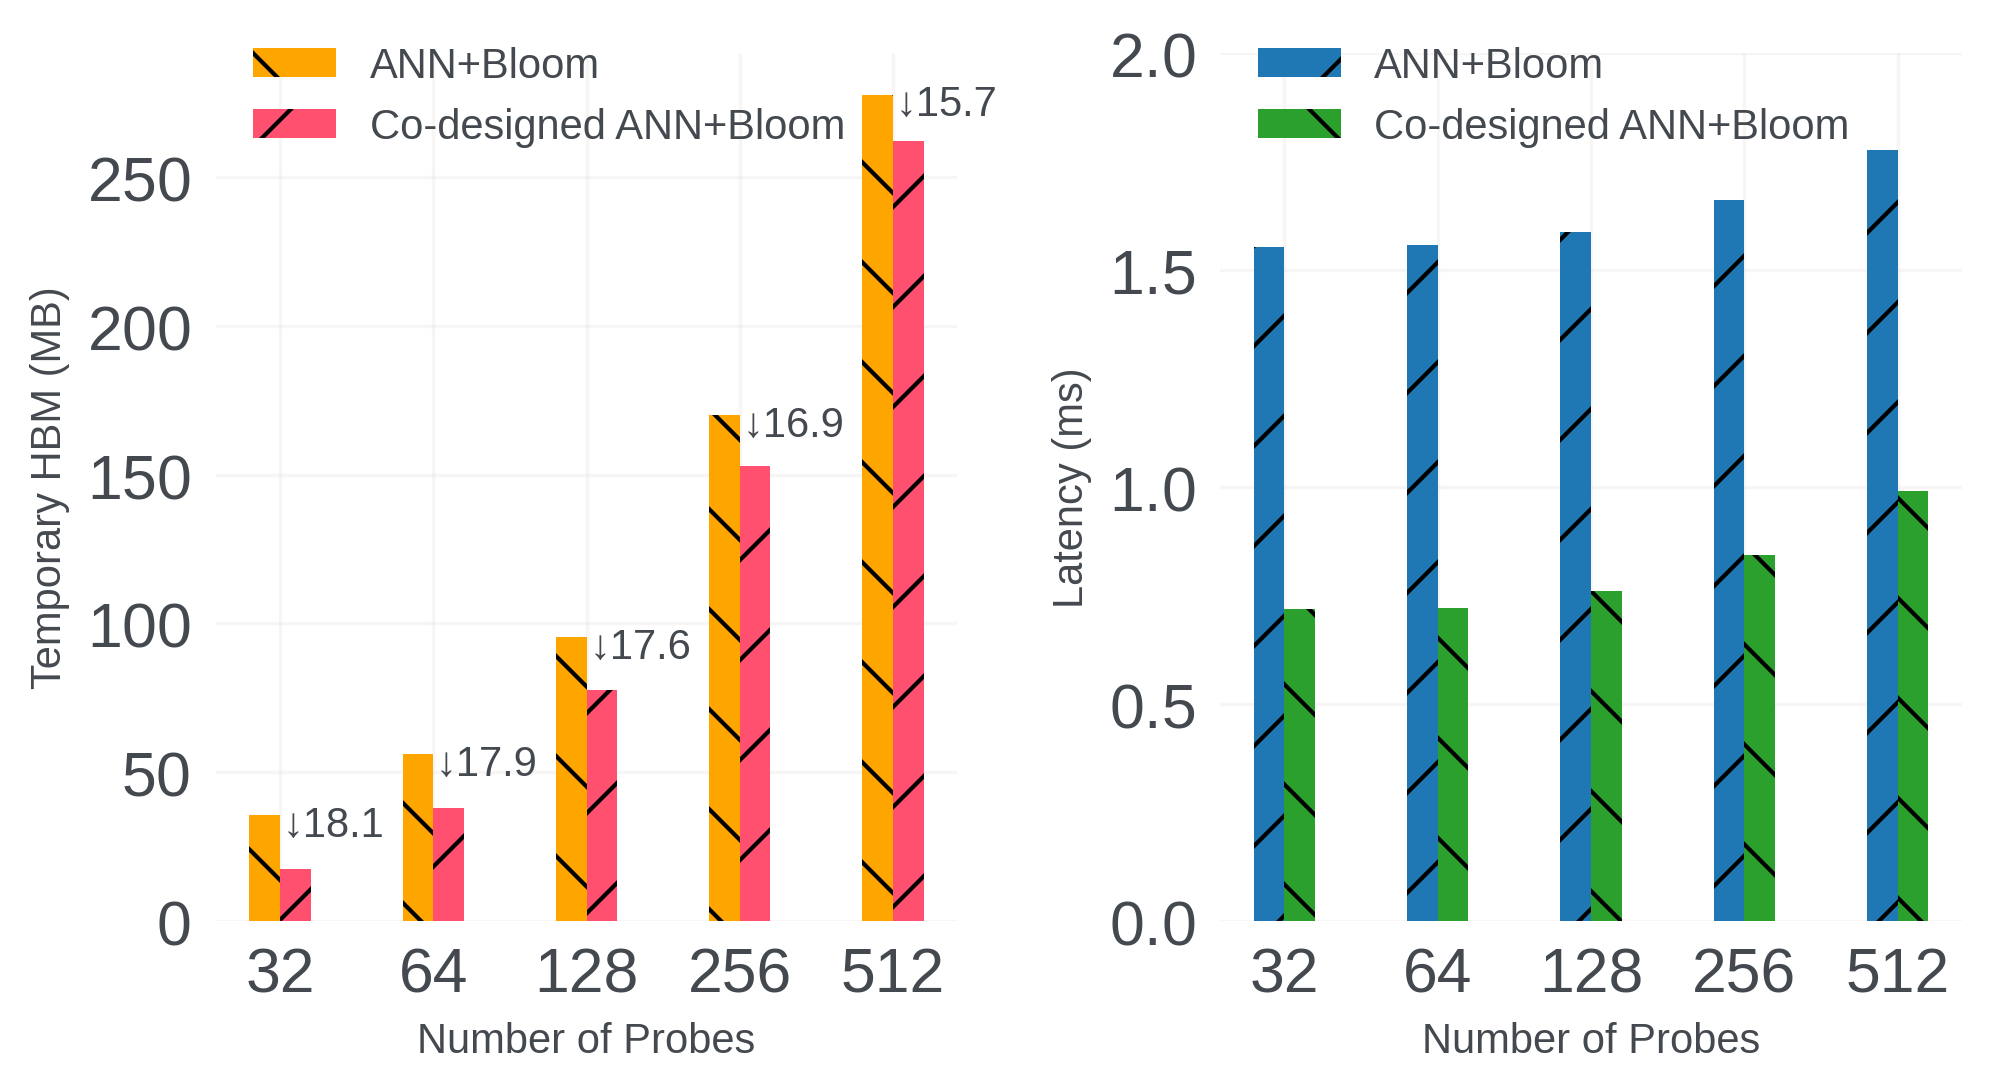
\includegraphics[width=0.5\textwidth]
    {figures/exp/co-designed.png}
    \caption{Latency and memory utilization comparison between co-designed ANN+Bloom and original ANN+Bloom.}
    \label{fig:bloom-joint}
\end{figure}

\subsubsection{Evaluation on ANN and filtering co-designed Index}
We evaluate co-designed index performance using a 20 million item dataset with 128-dimensional embeddings, comparing against a baseline that runs Bloom index separately and passes mask results to ANN. Figure \ref{fig:bloom-joint} shows GPU memory utilization and latency across probe counts. At probe=32, the baseline requires 35.6MB scratch memory (17.4MB for ANN, 18.2MB for Bloom index). Co-design reduces Bloom index scratch memory to 0.14MB, lowering total memory to 18.2MB while reducing latency from 1.55ms to 0.72ms. On average, co-design achieves $1.79\times$–$2.15\times$ latency improvement. As discussed, memory savings in this memory-bound scenario enable larger request batching and higher QPS.
  
\subsubsection{Evaluation on OverArch Scoring and Value Model}
\label{sec:634}
We evaluate OverArch and Value Model benefits by comparing recalls at different sizes, with ground truth from user-item interaction behaviors and probes set to 32. We report recalls for a major engagement event (E-Task) and consumption event (C-Task). The OverArch implements Mixture of Logits (MoL), while the Value Model applies rules validated through online A/B testing.
As shown in Table \ref{tab:recall-overarch}, adding scoring layers improves E-Task recall by 2.4–28.2 and C-Task recall by 0.6–1.12 across different sizes. While QPS only decreases from 1210 to 771, SilverTorch still achieves $15.11\times$ QPS speedup compared to service-based solutions.